\documentclass{article}

% Language setting
\usepackage{ctex}
\usepackage{listings}
\usepackage{fontspec}
\usepackage[framemethod=TikZ]{mdframed}

% Set page size and margins
% Replace `letterpaper' with `a4paper' for UK/EU standard size
\usepackage[letterpaper,top=2cm,bottom=2cm,left=3cm,right=3cm,marginparwidth=1.75cm]{geometry}

% Useful packages
\usepackage{amsmath}
\usepackage{amssymb}
\usepackage{graphicx}
\usepackage{float}
\usepackage{subcaption}
\usepackage[colorlinks=true, allcolors=blue]{hyperref}

\title{随机微分方程的轨道讨论}
\author{}

\begin{document}
\maketitle

\section{问题1}

\begin{mdframed} [%
	roundcorner=5pt,
	linecolor=gray!50,
	outerlinewidth=0.5pt,
	middlelinewidth=0.3pt, backgroundcolor=gray!2,
innertopmargin=\topskip, frametitle={问题1},
frametitlefont= \bfseries,frametitlerule=true,frametitlealignment =\raggedright\noindent,
frametitlerulewidth=.5pt, frametitlebackgroundcolor=gray!2,]
电脑生成多条布朗运动(BM)轨道。
\end{mdframed}

如果随机过程$\boldsymbol{X} = \{ X(t) ; t \geq 0 \}$ 是\textbf{布朗运动},则

\begin{itemize}
\item $\boldsymbol{X}$ 是独立增量过程;
\item $ \forall s,t > 0, X(s+t) - X(t) ~ N(0, c^2 t) $;
\item 轨道连续。
\end{itemize}

特别的,如果$\boldsymbol{X}$是\textbf{标准布朗运动(BM)},则$X(0) = 0, c = 1$。

基于以上对标准布朗运动的定义,电脑生成布朗运动轨道的算法如下:

\begin{itemize}
\item $\widehat{X}_0 = x_0$(此处$x_0 = 0$);
\item 确定一个极小的时间间隔$h$以及迭代次数$m$;
\item 迭代方程:$\forall k \in \mathbb{N},k < m$ ,有
$$
\widehat{X}_{(m+1)h} = \widehat{X}_{mh} + \sqrt{h}Z_k
$$
其中$\{Z_k;k \in \mathbb{N}\}$为一系列的满足正态分布的随机变量。
\end{itemize}

实际运行算法时,取$m = 10000, h = 0.001$, 生成10条轨道,最后算法生成的轨道如图\ref{fig:BM}所示。

\begin{figure}[H]
\centering
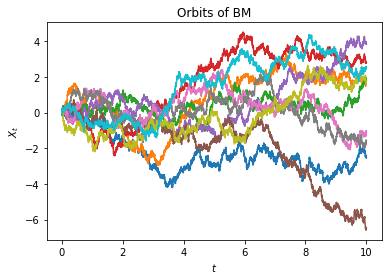
\includegraphics[width=0.6\textwidth]{figures/BM Orbit.png}
\caption{\label{fig:BM}标准布朗运动轨道}
\end{figure}

\section{问题2}

\begin{mdframed} [%
	roundcorner=5pt,
	linecolor=gray!50,
	outerlinewidth=0.5pt,
	middlelinewidth=0.3pt, backgroundcolor=gray!2,
innertopmargin=\topskip, frametitle={问题2},
frametitlefont= \bfseries,frametitlerule=true,frametitlealignment =\raggedright\noindent,
frametitlerulewidth=.5pt, frametitlebackgroundcolor=gray!2,]
设 $\boldsymbol{B}=\left\{\boldsymbol{B}_t ; \boldsymbol{t} \geq \mathbf{0}\right\}$ 为标准布朗运动, $\boldsymbol{X}=\left\{\boldsymbol{X}_{\boldsymbol{t}} ; \boldsymbol{t} \geq \mathbf{0}\right\}$ 为如下随机微分方程的解:
$$
\left\{\begin{array}{l}
d X_t=\alpha\left(v-X_t\right) d t+\sigma d B_t \\
X_0=x_0
\end{array}\right.$$
其中 $\alpha, v, \sigma, x_0$ 为常数。

(1) 用电脑生成 $X$ 的多条轨道;

(2) 探究不同的参数对轨道的影响;

(3) 用Monte Caro方法计算 $\boldsymbol{E}\left(\boldsymbol{X}_1\right), \boldsymbol{D}\left(\boldsymbol{X}_1\right)$
\end{mdframed}

\subsection{第1小问}

类似问题1的算法,生成满足问题2的随机微分方程的轨道的算法如下:

\begin{itemize}
\item $\widehat{X}_0 = x_0$;
\item 确定一个极小的时间间隔$h$以及迭代次数$m$;
\item 迭代方程:$\forall k \in \mathbb{N},k < m$ ,有
$$
\widehat{X}_{(m+1)h} = \widehat{X}_{mh} + \alpha h(v - \widehat{X}_{mh})  + \sigma \sqrt{h}Z_k
$$
其中$\{Z_k;k \in \mathbb{N}\}$为一系列的满足正态分布的随机变量。
\end{itemize}

在本小问中,实际运行算法时,取$m = 10000, h = 0.001$,同时取$x_0 = 0, \alpha = 2.0, v = 0.5, \sigma = 0.2$, 生成10条轨道,最后算法生成的轨道如图\ref{fig:SDE1}所示。

\begin{figure}[H]
\centering
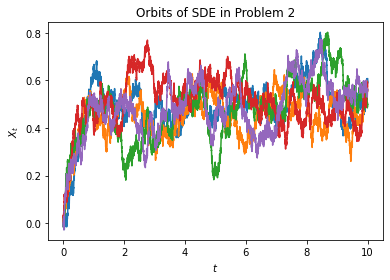
\includegraphics[width=0.6\textwidth]{figures/SDE1 Orbit1.png}
\caption{\label{fig:SDE1}问题二SDE轨道($\alpha = 2.0, v = 0.5, \sigma = 0.2, x_0 = 0 $)}
\end{figure}

\subsection{第2小问}

\subsubsection{探究$x_0$对轨道的影响}

下面探究$x_0$对轨道的影响,这里固定$\alpha = 2.0, v = 0.5, \sigma = 0.2$,选择$x_0 = 0$和$x_0 = 1$对轨道进行观察,具体的轨道如图\ref{fig:SDE1x0}所示。 

\begin{figure}[H]
    \centering
    \begin{minipage}[c]{0.48\textwidth}
        \centering
        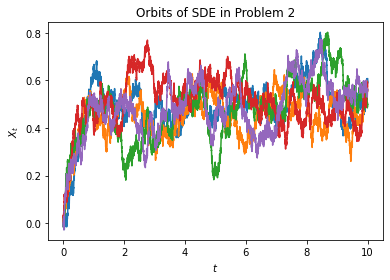
\includegraphics[height=0.2\textheight]{figures/SDE1 Orbit1.png}
        \subcaption{$x_0 = 0$}
    \end{minipage}
    \begin{minipage}[c]{0.48\textwidth}
        \centering
        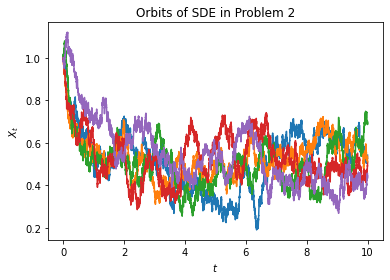
\includegraphics[height=0.2\textheight]{figures/SDE1 Orbit2.png}
        \subcaption{$x_0 = 1$}
    \end{minipage}
    \caption{探究$x_0$对轨道的影响($\alpha = 2.0, v = 0.5, \sigma = 0.2$)}
    \label{fig:SDE1x0}
\end{figure}

由图\ref{fig:SDE1x0}可知,$x_0$只影响了初始点的位置。

\subsubsection{探究$v$对轨道的影响}

下面探究$v$对轨道的影响,这里固定$x_0 = 0, \alpha = 2.0, \sigma = 0.2$,选择$v = 0.5$和$v = -0.5$对轨道进行观察,具体的轨道如图\ref{fig:SDE1v}所示。 

\begin{figure}[H]
    \centering
    \begin{minipage}[c]{0.48\textwidth}
        \centering
        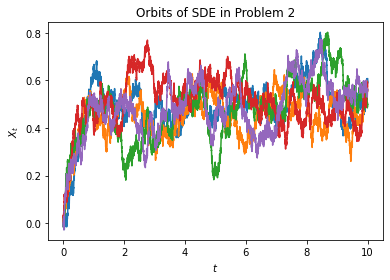
\includegraphics[height=0.2\textheight]{figures/SDE1 Orbit1.png}
        \subcaption{$v = 0.5$}
    \end{minipage}
    \begin{minipage}[c]{0.48\textwidth}
        \centering
        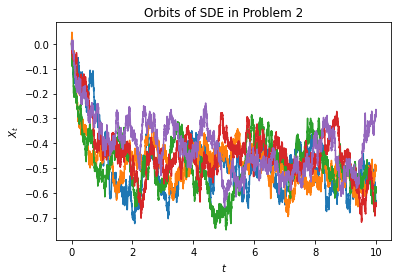
\includegraphics[height=0.2\textheight]{figures/SDE1 Orbit3.png}
        \subcaption{$v = -0.5$}
    \end{minipage}
    \caption{探究$x_0$对轨道的影响($x_0 = 0, \alpha = 2.0, \sigma = 0.2$)}
    \label{fig:SDE1v}
\end{figure}

由图\ref{fig:SDE1v}可知,$v$影响了轨道经过一段时间后收敛的区域范围(在$v$周围上下有少许浮动)。

\subsubsection{探究$\alpha, \sigma$对轨道的影响}

下面探究$\alpha, \sigma$对轨道的影响,这里固定$x_0 = 0, v = 0.5$,选择$(\alpha, \sigma) = (2.0, 0.2)$, $(\alpha, \sigma) = (2.0, 2.0)$, $(\alpha, \sigma) = (2.0, 5.0)$和$(\alpha, \sigma) = (-2.0, 0.2)$对轨道进行观察,具体的轨道如图\ref{fig:SDE1ab}所示。 

\begin{figure}[H]
    \centering
    \begin{minipage}[c]{0.45\textwidth}
        \centering
        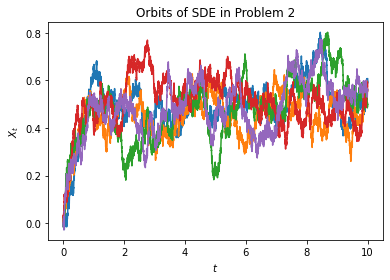
\includegraphics[width=0.95\textwidth]{figures/SDE1 Orbit1.png}
        \subcaption{$\alpha = 2.0, \sigma = 0.2$}
        \label{fig:SDE1ab-a}
    \end{minipage}
    \begin{minipage}[c]{0.45\textwidth}
        \centering
        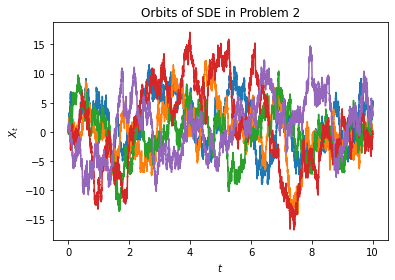
\includegraphics[width=0.95\textwidth]{figures/SDE1 Orbit4.png}
        \subcaption{$\alpha = 2.0, \sigma = 2.0$}
        \label{fig:SDE1ab-b}
    \end{minipage}
    \begin{minipage}[c]{0.45\textwidth}
        \centering
        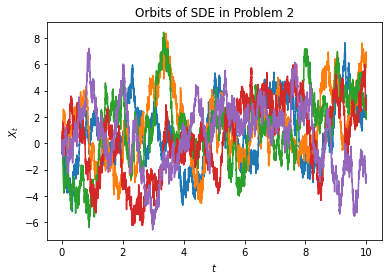
\includegraphics[width=0.95\textwidth]{figures/SDE1 Orbit5.png}
        \subcaption{$\alpha = 2.0, \sigma = 5.0$}
        \label{fig:SDE1ab-c}
    \end{minipage}
    \begin{minipage}[c]{0.45\textwidth}
        \centering
        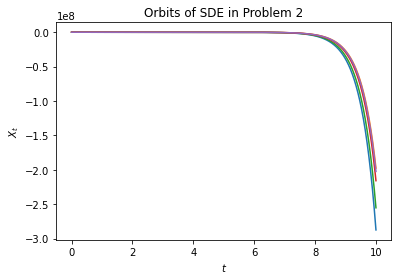
\includegraphics[width=0.95\textwidth]{figures/SDE1 Orbit6.png}
        \subcaption{$\alpha = -2.0, \sigma = 0.2$}
        \label{fig:SDE1ab-d}
    \end{minipage}
    \caption{探究$\alpha, \sigma$对轨道的影响($x_0 = 0, v = 0.5$)}
    \label{fig:SDE1ab}
\end{figure}

由图\ref{fig:SDE1ab}可知,$\alpha$和$\sigma$的相对大小会影响轨道是否可以在一段时间内收敛。

如图\ref{fig:SDE1ab-a}所示,当$\alpha > 0$且$\alpha >> \sigma$时,轨道逐渐稳定,可以在一段时间内收敛至$v$附近。

如图\ref{fig:SDE1ab-b}和图\ref{fig:SDE1ab-c}所示,当$\alpha= \sigma$或$\alpha<\sigma$时,轨道难以收敛,不断波动,且差值越大,上下波动的现象越明显。

如图\ref{fig:SDE1ab-d}所示,当$\alpha < 0$时,轨道无法收敛。


\subsection{第3小问}

在这一小问中,设定参数$\alpha = 2.0, \sigma = 0.2, v = 1.0, x_0 = 0$。

利用Monte Caro方法,模拟10000次轨道得到$\boldsymbol{E}(X_1)$和$\boldsymbol{E}(X_1^2)$,在设定参数情况下,$\boldsymbol{E}(X_1) = 0.433,\boldsymbol{E}(X_1^2) = 0.197$,详细代码见附录。

利用$\boldsymbol{D}(X_1) = \boldsymbol{E}(X_1^2) - \boldsymbol{E}^2(X_1)$,可得$\boldsymbol{D}(X_1) = 0.0095$

\section{问题3}

\begin{mdframed} [%
	roundcorner=5pt,
	linecolor=gray!50,
	outerlinewidth=0.5pt,
	middlelinewidth=0.3pt, backgroundcolor=gray!2,
innertopmargin=\topskip, frametitle={问题3},
frametitlefont= \bfseries,frametitlerule=true,frametitlealignment =\raggedright\noindent,
frametitlerulewidth=.5pt, frametitlebackgroundcolor=gray!2,]
设 $\boldsymbol{B}=\left\{\boldsymbol{B}_{\boldsymbol{t}} ; \boldsymbol{t} \geq \mathbf{0}\right\}$ 与 $\boldsymbol{W}=\left\{\boldsymbol{W}_{\boldsymbol{t}} ; \boldsymbol{t} \geq \mathbf{0}\right\}$ 为标准布朗运动, $\boldsymbol{X}=$ $\left(X_t, S_t\right)$ 为如下随机微分方程的解:
$$
\left\{\begin{array}{l}
d X_t=\alpha\left(v-X_t\right) d t+\sigma d B_t, \\
d S_t=\theta\left(X_t-S_t\right) d t+\hat{\sigma}_1 d B_t+\hat{\sigma}_2 d W_t \\
X_0=x_0, S_0=s_0
\end{array}\right.
$$
其中 $\alpha, v, \sigma, \theta, \widehat{\sigma}_1, \widehat{\sigma}_2, x_0, s_0$ 为常数。

(1) 用电脑生成 $(\boldsymbol{X}, \boldsymbol{S})$ 的多条轨道;

(2) 探究不同的参数对轨道的影响;

(3) 用Monte Caro方法计算 $\boldsymbol{E}\left(S_1\right), \boldsymbol{D}\left(S_1\right)$
\end{mdframed}

\subsection{第1小问}

类似问题1的算法,生成满足问题3的随机微分方程的轨道的算法如下:

\begin{itemize}
\item $\widehat{X}_0 = x_0$,$\widehat{S}_0 = s_0$;
\item 确定一个极小的时间间隔$h$以及迭代次数$m$;
\item 迭代方程:$\forall k \in \mathbb{N},k < m$ ,有
$$
\widehat{X}_{(m+1)h} = \widehat{X}_{mh} + \alpha (v - X_t) + \sigma \sqrt{h}Z_k \\
$$
$$
\widehat{S}_{(m+1)h} = \widehat{S}_{mh} + \theta h(\widehat{X}_{mh} - \widehat{S}_{mh}) + \hat{\sigma}_1 \sqrt{h}Z_k + \hat{\sigma}_2 \sqrt{h}W_k\\
$$
其中$\{Z_k;k \in \mathbb{N}\}$和$\{W_k;k \in \mathbb{N}\}$为系列的满足标准正态分布的随机变量。
\end{itemize}

在本小问中,实际运行算法时,取$m = 10000, h = 0.001$,同时取$x_0 = 10, s_0 = 12,\alpha = 2.0, v = 14.0, \sigma = 2.0, \theta = 2.0, \sigma_1 =  2.0, \sigma_2 = 2.0$,最后算法生成的轨道如图\ref{fig:SDE2}所示。

\begin{figure}[H]
\centering
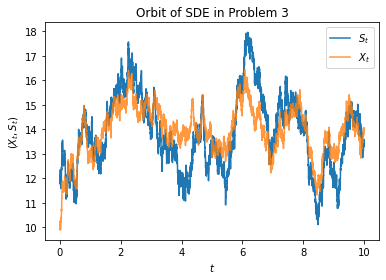
\includegraphics[width=0.6\textwidth]{figures/SDE2 Orbit1.png}
\caption{\label{fig:SDE2}问题三SDE轨道(第1小问给定条件下)}
\end{figure}

\subsection{第2小问}

由于在第二题中已经讨论过$x_0, v, \alpha, \sigma$对于轨道$\boldsymbol{X}_t$的影响,所以在此小问中不做赘述,下面主要探究$s_0, \theta, \hat{\sigma}_1, \hat{\sigma}_2$对于轨道$\boldsymbol{S}_t$的影响。

\subsubsection{探究$s_0$对轨道的影响}

下面探究$s_0$对轨道的影响,这里固定$x_0 = 10,\alpha = 2.0, v = 14.0, \sigma = 2.0, \theta = 2.0, \sigma_1 =  2.0, \sigma_2 = 2.0$,选择$s_0 = 10$和$x_0 = 20$对轨道进行观察,具体的轨道如图\ref{fig:SDE2s0}所示。 

\begin{figure}[H]
    \centering
    \begin{minipage}[c]{0.48\textwidth}
        \centering
        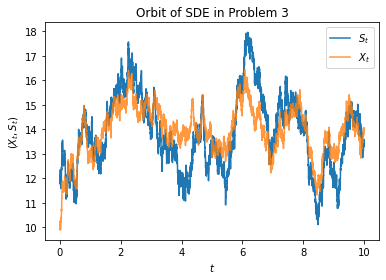
\includegraphics[height=0.2\textheight]{figures/SDE2 Orbit1.png}
        \subcaption{$s_0 = 12$}
    \end{minipage}
    \begin{minipage}[c]{0.48\textwidth}
        \centering
        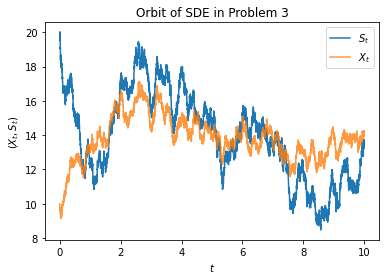
\includegraphics[height=0.2\textheight]{figures/SDE2 Orbit2.png}
        \subcaption{$s_0 = 20$}
    \end{minipage}
    \caption{探究$s_0$对轨道的影响(除$s_0$其他条件固定情况下)}
    \label{fig:SDE2s0}
\end{figure}

由图\ref{fig:SDE2s0}可知,$s_0$只影响了初始点的位置。

\subsubsection{探究$\theta, \hat{\sigma}_1, \hat{\sigma}_2$对轨道的影响}

下面探究$\theta, \hat{\sigma}_1, \hat{\sigma}_2$对轨道的影响,这里固定$x_0 = 10, s_0 = 12, \alpha = 2.0, v = 14.0, \sigma = 2.0$,选择$(\theta, \hat{\sigma}_1, \hat{\sigma}_2) = (2.0, 2.0, 2.0)$, $(\theta, \hat{\sigma}_1, \hat{\sigma}_2) = (5.0, 2.0, 2.0)$,$(\theta, \hat{\sigma}_1, \hat{\sigma}_2) = (2.0, 0.2, 0.2)$和$(\theta, \hat{\sigma}_1, \hat{\sigma}_2) = (-2.0,2.0, 2.0)$对轨道进行观察,具体的轨道如图\ref{fig:SDE2ts}所示。 

\begin{figure}[H]
    \centering
    \begin{minipage}[c]{0.45\textwidth}
        \centering
        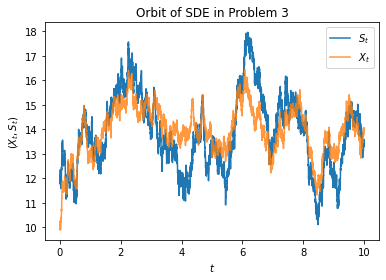
\includegraphics[width=0.95\textwidth]{figures/SDE2 Orbit1.png}
        \subcaption{$\theta = 2.0, \hat{\sigma}_1 = 2.0, \hat{\sigma}_2 = 2.0$}
        \label{fig:SDE2ts-a}
    \end{minipage}
    \begin{minipage}[c]{0.45\textwidth}
        \centering
        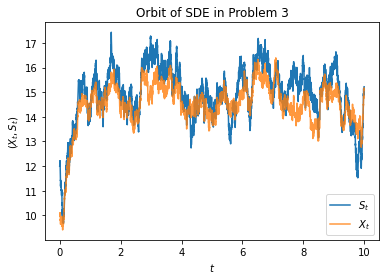
\includegraphics[width=0.95\textwidth]{figures/SDE2 Orbit3.png}
        \subcaption{$\theta = 5.0, \hat{\sigma}_1 = 2.0, \hat{\sigma}_2 = 2.0$}
        \label{fig:SDE2ts-b}
    \end{minipage}
    \begin{minipage}[c]{0.45\textwidth}
        \centering
        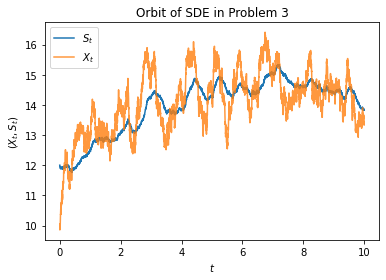
\includegraphics[width=0.95\textwidth]{figures/SDE2 Orbit4.png}
        \subcaption{$\theta = 2.0, \hat{\sigma}_1 = 0.2, \hat{\sigma}_2 = 0.2$}
        \label{fig:SDE2ts-c}
    \end{minipage}
    \begin{minipage}[c]{0.45\textwidth}
        \centering
        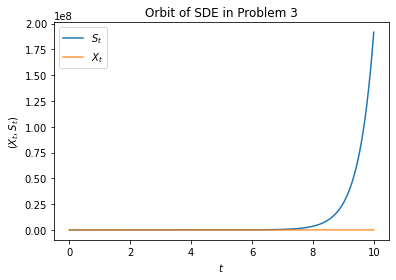
\includegraphics[width=0.95\textwidth]{figures/SDE2 Orbit5.png}
        \subcaption{$\theta = -2.0, \hat{\sigma}_1 = 2.0, \hat{\sigma}_2 = 2.0$}
        \label{fig:SDE2ts-d}
    \end{minipage}
    \caption{探究$\theta, \hat{\sigma}_1, \hat{\sigma}_2$对轨道的影响}
    \label{fig:SDE2ts}
\end{figure}

由图\ref{fig:SDE2ts}可知,$\theta$和$\hat{\sigma}_1, \hat{\sigma}_2$的相对大小会影响轨道$\boldsymbol{S}_t$和轨道$\boldsymbol{X}_t$的相似性。

比较图\ref{fig:SDE2ts-a}和图\ref{fig:SDE2ts-b},当$\hat{\sigma}_1, \hat{\sigma}_2$固定时,随着$\theta$的增大,$\boldsymbol{S}_t$逐渐向轨道$\boldsymbol{X}_t$靠拢,相似度越来越高。

比较图\ref{fig:SDE2ts-a}和图\ref{fig:SDE2ts-c},当$\theta$固定时,随着$\hat{\sigma}_1, \hat{\sigma}_2$的减少,轨道$\boldsymbol{S}_t$的波动越来越小,且与轨道$\boldsymbol{X}_t$的相似性越来越低。

如图\ref{fig:SDE2ts-d}所示,当$\theta < 0$时,轨道$\boldsymbol{S}_t$无法收敛且与$\boldsymbol{X}_t$的差距随着时间推移越来越大。

\subsection{第3小问}

在这一小问中,设定参数$x_0 = 10, s_0 = 12,\alpha = 2.0, v = 14.0, \sigma = 2.0, \theta = 2.0, \sigma_1 =  2.0, \sigma_2 = 2.0$。

利用Monte Caro方法,模拟10000次轨道得到$\boldsymbol{E}(S_1)$和$\boldsymbol{E}(S_1^2)$,在设定参数情况下,$\boldsymbol{E}(S_1) = 13.780,\boldsymbol{E}(S_1^2) = 258.044$,详细代码见附录。

利用$\boldsymbol{D}(S_1) = \boldsymbol{E}(S_1^2) - \boldsymbol{E}^2(S_1)$,可得$\boldsymbol{D}(S_1) = 68.162$

\section{感想}

在这次大作业中,我通过Python软件依照要求绘制了不同的轨道,从一方面来说,这加深了我对随机微分方程(SDE)的理解,从另一方面来说,这也加强了我对python编程的理解。在讨论作业之中随机微分方程的轨道时,我认识到要同时考虑趋势项和波动项。对于趋势项,它是确定性函数,也是历史数据对应的部分,这个部分可以大体展现轨道的总体形状;对于波动项,这个部分则是反映了轨道的随机性。除此之外,在不同的情况下,也需要分析两个部分的大小关系对轨道的影响。随机项参数较大时,轨道的波动较为明显;波动项和趋势项参数持平时,两者都会对最终轨道有一定作用,波动相比于前一种情况有所减缓但依旧明显;而趋势项参数较大时,轨道展现的是相对确定的函数曲线再叠加上小范围的波动。在实际问题中,判断当前随机微分方程所处的“状态”(即趋势明显或波动明显,对应金融中股票市场的牛市熊市和震荡盘)是极为重要的。

最后,我想说,作为一名工科的学生,我在之前只学过概率统计这门与统计相关的课,感谢熊德文老师的授课以及以及助教的无私奉献,使我能够对随机过程的相关理论有所理解。未来我也会努力将所学到的理论知识与自己的专业领域有机结合。再次对您们表示衷心的感谢。

\section{附录}

\subsection{问题1代码}

\begin{lstlisting}[language = python, numbers=left, numberstyle=\tiny, keywordstyle=\color{blue!70}, commentstyle=\color{red!50!green!50!blue!50},frame=shadowbox,rulesepcolor=\color{red!20!green!20!blue!20},basicstyle=\ttfamily]
import numpy as np
from matplotlib import pyplot as plt
import random
import datetime
random.seed(datetime.datetime.now())

def BM(T, m, n): 
    # n: sample path的数目
    # m: 时间离散的步数
    # T: 仿真的终止时间
    
    h = T / m # 时间步长
    
    Z = np.random.normal(0.0, 1.0, (n, m)) # 标准正态分布变量
    
    X = np.zeros((n, m + 1)) # 存储n条路径的矩阵
    
    X[:, 0] = x0 # 初始化
    
    for i in range(m):
        # 迭代:矩阵化实现
        X[:, i + 1] = X[:, i] + np.sqrt(h) * Z[:, i]
    
    return X

# 实验
x0 = 0
T, m, n = 10.0, 10000, 10

X = BM(T, m, n)

# 时间格点
t_grid = np.linspace(0, T, m + 1)

# 展示结果
for i in range(n):
    plt.plot(t_grid, X[i, :])

plt.xlabel('$t$')
plt.ylabel('$X_t$')
plt.title('Orbits of BM')
plt.show()
\end{lstlisting}

\subsection{问题2代码}

\begin{lstlisting}[language = python, numbers=left, numberstyle=\tiny, keywordstyle=\color{blue!70}, commentstyle=\color{red!50!green!50!blue!50},frame=shadowbox,rulesepcolor=\color{red!20!green!20!blue!20},basicstyle=\ttfamily]
def SDE_ez(T, m, n): 
    # n: sample path的数目
    # m: 时间离散的步数
    # T: 仿真的终止时间
    
    h = T / m # 时间步长
    
    Z = np.random.normal(0.0, 1.0, (n, m)) # 标准正态分布变量
    
    X = np.zeros((n, m + 1)) # 存储n条路径的矩阵
    
    X[:, 0] = x0 # 初始化
    
    for i in range(m):
        # 迭代:矩阵化实现
        X[:, i + 1] = X[:, i] + alpha * (mu - X[:, i]) * h 
        + sigma * np.sqrt(h) * Z[:, i]
    
    return X

# 实验
x0 = 0
T, m, n = 10.0, 10000, 5
alpha, mu, sigma = 2.0, 0.5, 0.2
X = SDE_ez(T, m, n)
su = 0
su2 = 0

# 时间格点
t_grid = np.linspace(0, T, m + 1)

# 计算期望和方差
for i in range(n):
    su += X[i, m]
    su2 += X[i, m] * X[i, m]
avg = su / n
avg2 = su2 / n
d = avg2 - avg * avg

# 展示结果
for i in range(n):
    plt.plot(t_grid, X[i, :])

plt.xlabel('$t$')
plt.ylabel('$X_t$')
plt.title('Orbits of SDE in Problem 2')
plt.show()
\end{lstlisting}

\subsection{问题3代码}

\begin{lstlisting}[language = python, numbers=left, numberstyle=\tiny, keywordstyle=\color{blue!70}, commentstyle=\color{red!50!green!50!blue!50},frame=shadowbox,rulesepcolor=\color{red!20!green!20!blue!20},basicstyle=\ttfamily]
def SDE_hd(T, m, n): 
    # n: sample path的数目
    # m: 时间离散的步数
    # T: 仿真的终止时间
    
    h = T / m # 时间步长
    
    Z = np.random.normal(0.0, 1.0, (n, m)) # 标准正态分布变量
    ZZ = np.random.normal(0.0, 1.0, (n, m)) # 标准正态分布变量
    
    X = np.zeros((n, m + 1)) # 存储n条路径的矩阵
    S = np.zeros((n, m + 1)) # 存储n条路径的矩阵
    
    X[:, 0] = x0 # 初始化
    S[:, 0] = s0 # 初始化
    
    for i in range(m):
        # 迭代:矩阵化实现
        X[:, i + 1] = X[:, i] + alpha * (mu - X[:, i]) * h 
        + sigma * np.sqrt(h) * Z[:, i]
        S[:, i + 1] = S[:, i] + theta * (X[:, i] - S[:, i]) * h 
        + sigma_1 * np.sqrt(h) * Z[:, i] 
        + sigma_2 * np.sqrt(h) * ZZ[:, i]
    
    return X, S

# 实验
x0 = 10
s0 = 12
T, m, n = 1.0, 1000, 10000
alpha, mu, sigma = 2.0, 14.0, 2.0
theta, sigma_1, sigma_2 = 2.0, 2.0, 2.0
su = 0
su2 = 0
X, S = SDE_hd(T, m, n)

# 时间格点
t_grid = np.linspace(0, T, m + 1)

# 计算期望和方差
for i in range(n):
    su += S[i, m]
    su2 += S[i, m] * S[i, m]
avg = su / n
avg2 = su2 / n
d = avg2 - avg * avg

# 展示结果
for i in range(n):    
    plt.plot(t_grid, S[i, :], label='$S_t$')
    
for i in range(n):
    plt.plot(t_grid, X[i, :], alpha = 0.8, label='$X_t$')

plt.xlabel('$t$')
plt.ylabel('$(X_t, S_t)$')
plt.legend()
plt.title('Orbit of SDE in Problem 3')
plt.show()
\end{lstlisting}












% \subsection{How to include Figures}

% \begin{figure}
% \centering
% \includegraphics[width=0.3\textwidth]{frog.jpg}
% \caption{\label{fig:frog}This frog was uploaded via the file-tree menu.}
% \end{figure}

% \subsection{How to add Tables}

% Use the table and tabular environments for basic tables --- see Table~\ref{tab:widgets}, for example. For more information, please see this help article on \href{https://www.overleaf.com/learn/latex/tables}{tables}. 

% \begin{table}
% \centering
% \begin{tabular}{l|r}
% Item & Quantity \\\hline
% Widgets & 42 \\
% Gadgets & 13
% \end{tabular}
% \caption{\label{tab:widgets}An example table.}
% \end{table}

% \subsection{How to add Comments and Track Changes}

% Comments can be added to your project by highlighting some text and clicking ``Add comment'' in the top right of the editor pane. To view existing comments, click on the Review menu in the toolbar above. To reply to a comment, click on the Reply button in the lower right corner of the comment. You can close the Review pane by clicking its name on the toolbar when you're done reviewing for the time being.

% Track changes are available on all our \href{https://www.overleaf.com/user/subscription/plans}{premium plans}, and can be toggled on or off using the option at the top of the Review pane. Track changes allow you to keep track of every change made to the document, along with the person making the change. 

% \subsection{How to add Lists}

% You can make lists with automatic numbering \dots

% \begin{enumerate}
% \item Like this,
% \item and like this.
% \end{enumerate}
% \dots or bullet points \dots
% \begin{itemize}
% \item Like this,
% \item and like this.
% \end{itemize}

% \subsection{How to change the margins and paper size}

% Usually the template you're using will have the page margins and paper size set correctly for that use-case. For example, if you're using a journal article template provided by the journal publisher, that template will be formatted according to their requirements. In these cases, it's best not to alter the margins directly.

% If however you're using a more general template, such as this one, and would like to alter the margins, a common way to do so is via the geometry package. You can find the geometry package loaded in the preamble at the top of this example file, and if you'd like to learn more about how to adjust the settings, please visit this help article on \href{https://www.overleaf.com/learn/latex/page_size_and_margins}{page size and margins}.



\end{document}